%! Author = adnansiddiquei
%! Date = 08/03/2024

\section{Experimentation, Profiling and Optimisation}\label{sec:profiling}
\begin{figure}[t]
\centering
\begin{subfigure}{0.9\textwidth}
  \centering
  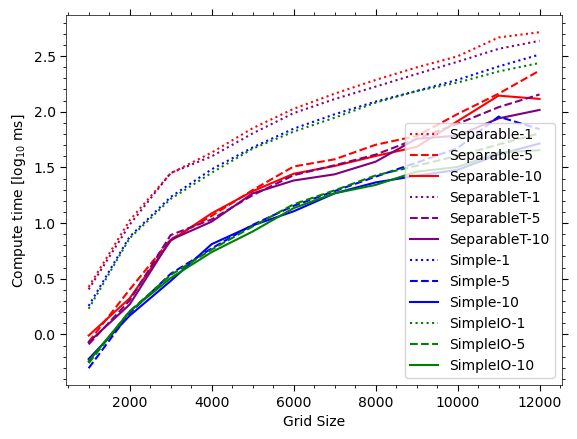
\includegraphics[width=.8\linewidth]{./figures/convolutions}
  \caption{A figure showing the compute time for 4 of the convolution methods for counting neighbours.
        The colour of the line indicates the method used, and the line style (dotted, dashed, solid) indicates the number
        OpenMP threads used (1, 5 and 10 respectively).
        Only 1 MPI rank was used.
        The x-axis shows the size of one dimension of the square grid.
        The Simple and Separable methods are as described in \eqref{subsec:domain-decomp} and the SimpleIO method is
        as described in \eqref{subsec:hiding-comms})
        The SeparableT method is the Separable method done in 2 horizontal passes with a transpose in between, except
        the time on the graph is just the compute time to repeat the first horizontal pass twice (for simplicity).}
  \label{fig:convolutions}
\end{subfigure}%
\hfill
\begin{subfigure}{0.9\textwidth}
  \centering
  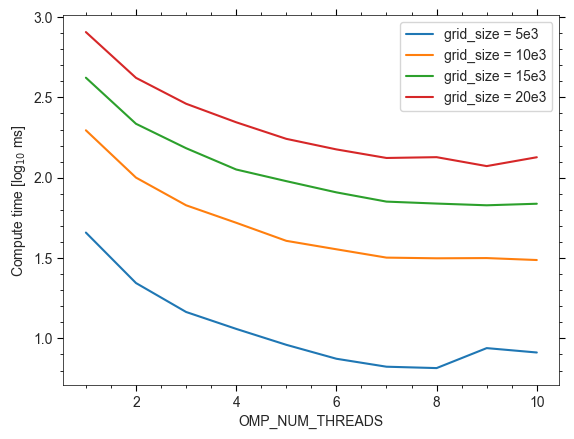
\includegraphics[width=0.8\linewidth]{./figures/simpleio}
  \caption{A figure showing how the compute time varies for the SimpleIO method as the number of OMP threads is changed.
    1 MPI rank was used, and compute time was averaged over 3 runs.}
  \label{fig:simpleio}
\end{subfigure}
\caption{Performance testing results for the various convolution methods for counting neighbours.}
\label{fig:conv}
\end{figure}

\begin{figure}[t]
\centering
\begin{subfigure}{0.9\textwidth}
  \centering
  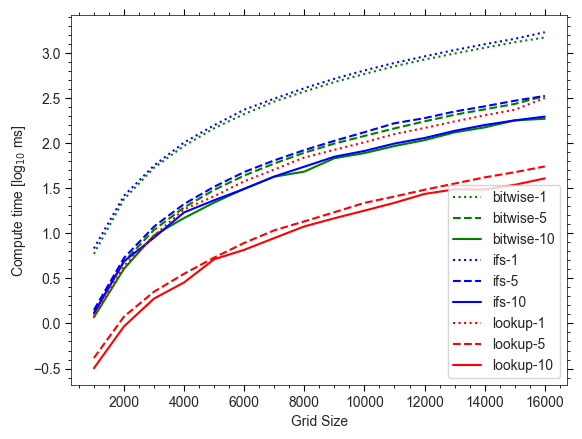
\includegraphics[width=.8\linewidth]{./figures/transitions}
  \caption{A figure showing the compute time (the time taken to update the entire grid once) for the 3 the update methods
    discussed in Section \eqref{subsec:update-grid}.
    The colour of the line indicates the method used, and the line style (dotted, dashed, solid) indicates the number
    OpenMP threads used (1, 5 and 10 respectively).
    Only 1 MPI rank was used and the compute time was averaged over 3 runs.}
  \label{fig:transitions}
\end{subfigure}%
\hfill
\begin{subfigure}{0.9\textwidth}
  \centering
  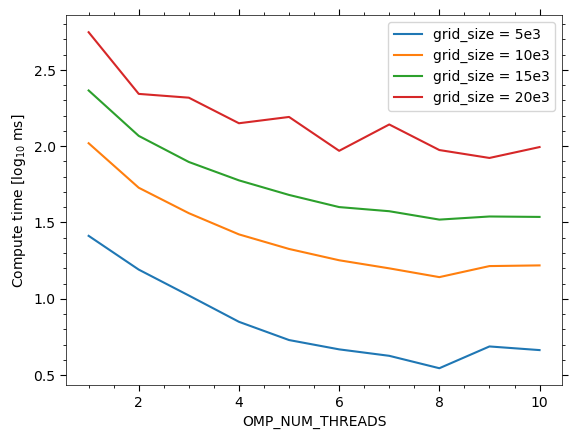
\includegraphics[width=0.8\linewidth]{./figures/lookup}
  \caption{A figure showing how the compute time varies for the updating the grid using the lookup method as the number
    of OMP threads is changed.
    1 MPI rank was used, and compute time was averaged over 5 runs.}
  \label{fig:lookup}
\end{subfigure}
\caption{Performance testing results for the various convolution methods for counting neighbours.}
\label{fig:trans}
\end{figure}

\begin{figure}[t]
\centering
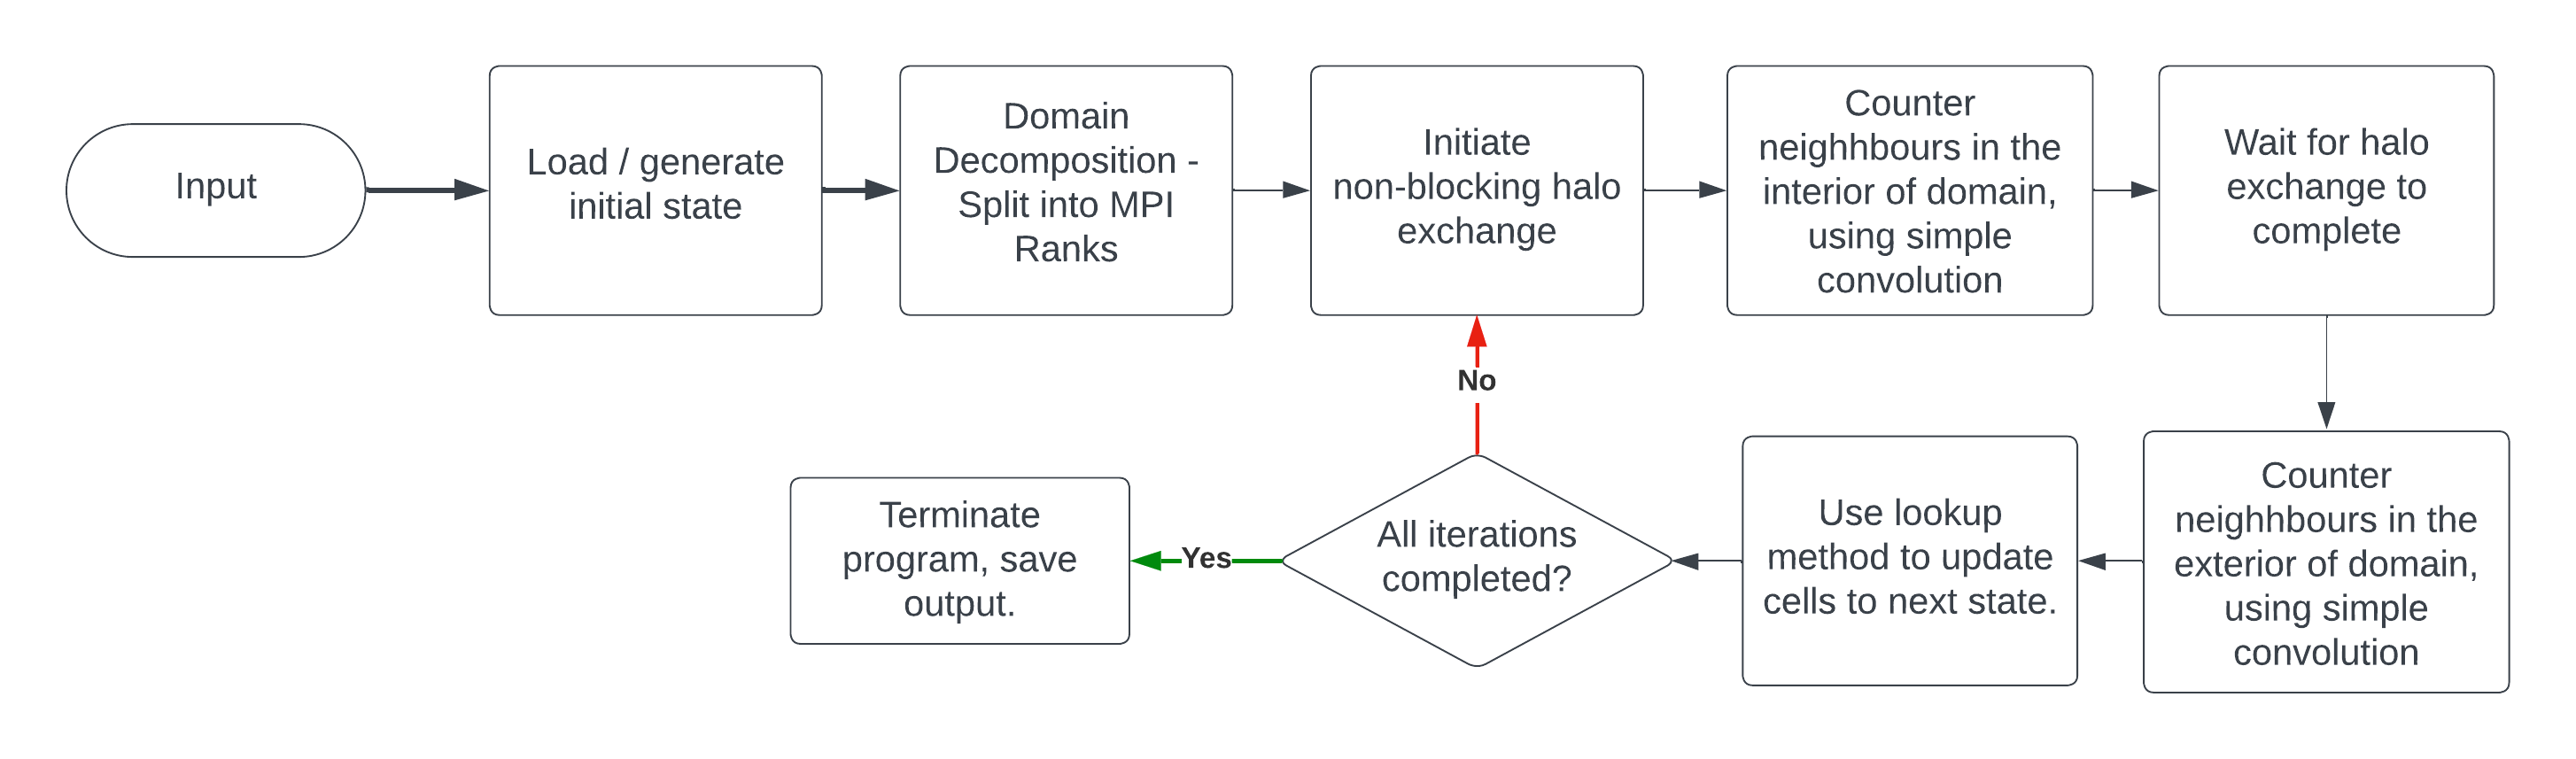
\includegraphics[width=0.85\textwidth]{./figures/flowchat-2}
\caption{An updated version of Fig.\eqref{fig:high-level-flowchart} with the conclusions from the experimentation
and profiling.}
\label{fig:flowhcart-2}
\end{figure}

\begin{figure}[t]
\centering
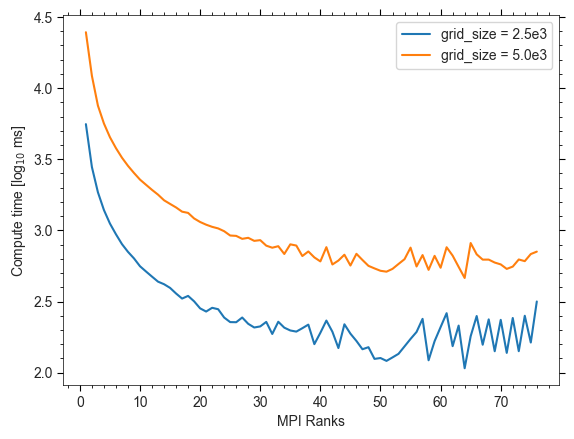
\includegraphics[width=0.9\textwidth]{./figures/mpi_hpc}
\caption{A plot of the compute time for the full simulation on a singular Icelake node (76 cores).
    The number of MPI ranks was varied but the OMP thread count was kept at 1.
    The compute time was averaged over 2 runs for grid sizes of $5 \times 10^{3}$ and $2.5 \times 10^{3}$ as they evolved
    over 200 generations.}
\label{fig:mpi_hpc}
\end{figure}

\begin{figure}[t]
\centering
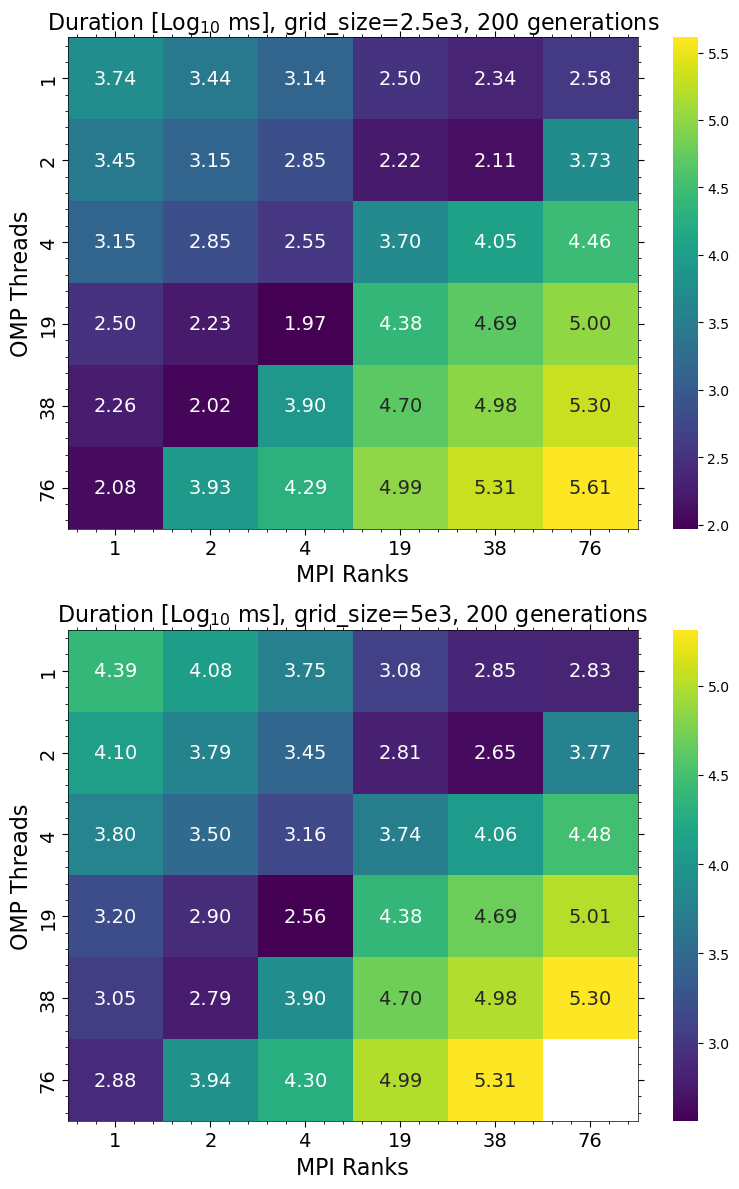
\includegraphics[width=0.8\textwidth]{./figures/mpi_vs_omp_hpc}
\caption{Heatmaps of the $Log_{10}(duration)$ for the full simulation on a singular Icelake node (76 cores).
    Both the number of MPI ranks and OMP threads were varied, with the diagonal (going from the bottom left to the top right)
    representing the full usage configurations of the node (where the number of MPI ranks and OMP threads multiplied to 76).
    The compute time was averaged over 2 runs}
\label{fig:mpi_vs_omp_hpc}
\end{figure}

This section discusses the experimentation and profiling of the different methods discussed in Section \eqref{sec:prototyping}.
Experimentation to decide algorithmic choices (which convolution Section~\eqref{subsec:domain-decomp}, and update method
Section~\eqref{subsec:update-grid} to use) was done on a Macbook M1 Pro (see Appendix~\eqref{app:macbook-specs} for specs).
Following the implementation of these decisions, the optimal algorithm was tested on a singular Icelake node to determine
the optimal number of MPI ranks and OMP threads to use for the full simulation.

\subsection{Profiling the Convolution Methods}\label{subsec:prof-conv}
Fig.\eqref{fig:convolutions} shows the compute time across 4 different convolution methods for counting neighbours
and how they scale with \inlinecode{grid_size} and \inlinecode{OMP_NUM_THREADS}.
The first observation is that both the simple methods are faster than both of the separable methods, which is
at face value, unexpected.
Furthermore, there is a negligible difference in speed between the Simple and SimpleIO method which is a positive
outcome which means the SimpleIO method is a good candidate for hiding communication overheads, as the vast majority
of the computation can be done while waiting for the communication to complete.
OpenMP was used to parallelise the convolution methods, as such, the Figure illustrates the compute times for a variety
of thread counts.

Loop unrolling was implemented in all of these convolutions, the kernel was applied
to the grid manually rather than having an additional loop (0 to 8) which applied the kernel.
Experimentally, this was found to yield about a 2.5x speedup (for the sake of brevity, no figures were generated to
supplement this conclusion).
Additionally, all of the double nested loops (which looped over the rows and columns of the grids) were parallelised
using the OMP \inlinecode{parallel for collapse} clause which allowed OMP to collapse and parallelise the
nested loops.

Fig.\eqref{fig:simpleio} illustrates how the SimpleIO method parallelises as the thread count is increased.
As expected, it shows diminishing returns, with the compute time flattening out as the thread count increases.

\subsection{Profiling the Update Methods}\label{subsec:prof-trans}
Fig.\eqref{fig:transitions} explores the update methods discussed in Section \eqref{subsec:update-grid}, with a
clear conclusion that the lookup method is the fastest, and as expected, the \inlinecode{if} method is the slowest.
This makes sense, due to the (effectively) random nature of the simulation, the CPU will have little success
in branch predictions, contributing to the slowness of the \inlinecode{if} method.
The frequent lookup in an 18-length array is relatively inexpensive compared to frequent branching.

Similar to Fig.\eqref{fig:simpleio}, Fig.\eqref{fig:lookup} shows that the lookup method for updating the grid starts
to show diminishing returns in performance after about 8 OMP threads have been created.

\subsection{Algorithm Conclusions}\label{subsec:interim-conclusions}
Given the above results, the SimpleIO and lookup methods are the best candidates for the neighbour counting and grid
updating algorithms respectively.
The SimpleIO can be used to hide communication overheads effectively and the lookup method is the fastest way to
update the grid, Fig~\eqref{fig:flowhcart-2} shows an updated flowchart of the overall algorithm.
These conclusions are likely transferable to other architectures (although the exact relative speed differences will
likely differ from chip to chip), and so these conclusions were not re-evaluated on the Icelake node.
It is likely that for the M1 Pro, the bottleneck at roughly 8 OMP threads is due to memory constraints rather
than the algorithm itself not parallelising well, given that the datasets used in the simulation are large enough
to completely fill L1 and shared L2 caches.

Additionally, the optimal domain decomposition was not explored due to time constraints, row-wise decomposition was implemented
for the sake of simplicity and it was preferred over column-wise decomposition to reduce non-contiguous data transfer
in the halo exchange.

\subsection{MPI Ranks and OMP Threads}\label{subsec:mpi-omp}
With the conclusions from Section~\eqref{subsec:interim-conclusions} implemented this section explores the dynamic of
the number of MPI ranks and OMP threads on the compute time.

Fig.\eqref{fig:mpi_hpc} shows the compute time for the full simulation on a singular Icelake node as the number of MPI
ranks is varied.
The compute time sharply decreases as the number of MPI ranks is increased, but tapers off at around 40 MPI ranks,
yielding diminishing returns following this point.
Figure~\eqref{fig:mpi_vs_omp_hpc} takes this analysis further and plots a heatmap of the compute time for the full
simulation as the number of MPI ranks and OMP threads are both varied.
As expected, generally the best performance was achieved on the full usage diagonal of the heatmap, where the number of
MPI ranks and OMP threads multiplied to 76 (the number of cores on the Icelake node), with an interesting exception at
19 ranks with 4 threads.
Another observation is that upper left triangle is preferred over the lower right triangle, i.e.,
configurations resulting in under-utilisation of the node were preferred over configurations resulting in over-utilisation
(hyper-threading).
This is likely due to the overheads of managing additional threads and ranks.
In fact, almost identical performance is seen across both grid sizes in the over-utilisation region.
The compute times in this region are a whole 2 magnitudes larger than the compute times in the full usage region indicating
the effects of too many ranks and threads.

There was, however, a consistent winner across both grid sizes and this was the 4 rank and 19 thread configuration.








